\begin{frame}{LoRa Modulation Technique: \alert{Chirp Spread Spectrum} (\alert{CSS})}
  \alert{Chirp Spread Spektrum} or \alert{CSS} for short is a modulation technique where \alert{sinusoidal} signals with over time \alert{raising (\textcolor{fh-ooe-red}{up-chirp})} or \alert{falling (\textcolor{fh-ooe-red}{down-chirp}) frequencies} are used.
  \begin{center}
    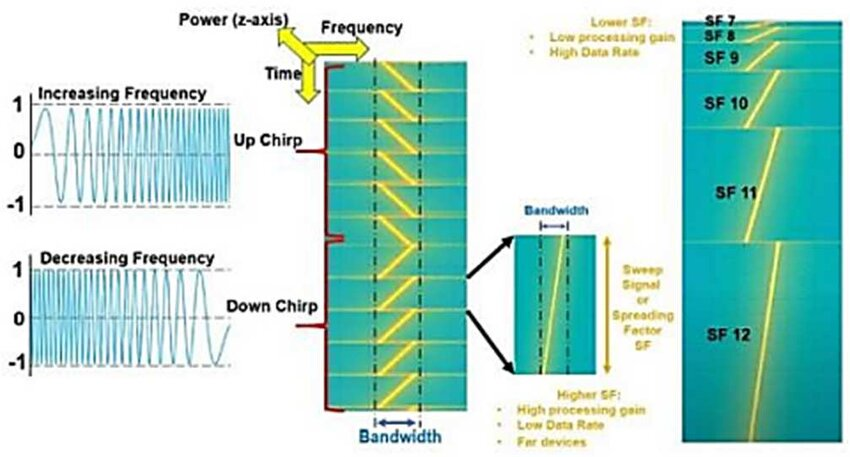
\includegraphics[width=0.7\textwidth]{material/LoRa-Chirp-Spread-Spectrum-Illustration-13.png}
  \end{center}
\end{frame}
